
%% bare_conf.tex
%% V1.4b
%% 2015/08/26
%% by Michael Shell
%% See:
%% http://www.michaelshell.org/
%% for current contact information.
%%
%% This is a skeleton file demonstrating the use of IEEEtran.cls
%% (requires IEEEtran.cls version 1.8b or later) with an IEEE
%% conference paper.
%%
%% Support sites:
%% http://www.michaelshell.org/tex/ieeetran/
%% http://www.ctan.org/pkg/ieeetran
%% and
%% http://www.ieee.org/

%%*************************************************************************
%% Legal Notice:
%% This code is offered as-is without any warranty either expressed or
%% implied; without even the implied warranty of MERCHANTABILITY or
%% FITNESS FOR A PARTICULAR PURPOSE! 
%% User assumes all risk.
%% In no event shall the IEEE or any contributor to this code be liable for
%% any damages or losses, including, but not limited to, incidental,
%% consequential, or any other damages, resulting from the use or misuse
%% of any information contained here.
%%
%% All comments are the opinions of their respective authors and are not
%% necessarily endorsed by the IEEE.
%%
%% This work is distributed under the LaTeX Project Public License (LPPL)
%% ( http://www.latex-project.org/ ) version 1.3, and may be freely used,
%% distributed and modified. A copy of the LPPL, version 1.3, is included
%% in the base LaTeX documentation of all distributions of LaTeX released
%% 2003/12/01 or later.
%% Retain all contribution notices and credits.
%% ** Modified files should be clearly indicated as such, including  **
%% ** renaming them and changing author support contact information. **
%%*************************************************************************


% *** Authors should verify (and, if needed, correct) their LaTeX system  ***
% *** with the testflow diagnostic prior to trusting their LaTeX platform ***
% *** with production work. The IEEE's font choices and paper sizes can   ***
% *** trigger bugs that do not appear when using other class files.       ***                          ***
% The testflow support page is at:
% http://www.michaelshell.org/tex/testflow/



\documentclass[conference]{IEEEtran}
% Some Computer Society conferences also require the compsoc mode option,
% but others use the standard conference format.
%
% If IEEEtran.cls has not been installed into the LaTeX system files,
% manually specify the path to it like:
% \documentclass[conference]{../sty/IEEEtran}





% Some very useful LaTeX packages include:
% (uncomment the ones you want to load)


% *** MISC UTILITY PACKAGES ***
%
%\usepackage{ifpdf}
% Heiko Oberdiek's ifpdf.sty is very useful if you need conditional
% compilation based on whether the output is pdf or dvi.
% usage:
% \ifpdf
%   % pdf code
% \else
%   % dvi code
% \fi
% The latest version of ifpdf.sty can be obtained from:
% http://www.ctan.org/pkg/ifpdf
% Also, note that IEEEtran.cls V1.7 and later provides a builtin
% \ifCLASSINFOpdf conditional that works the same way.
% When switching from latex to pdflatex and vice-versa, the compiler may
% have to be run twice to clear warning/error messages.






% *** CITATION PACKAGES ***
%
%\usepackage{cite}
% cite.sty was written by Donald Arseneau
% V1.6 and later of IEEEtran pre-defines the format of the cite.sty package
% \cite{} output to follow that of the IEEE. Loading the cite package will
% result in citation numbers being automatically sorted and properly
% "compressed/ranged". e.g., [1], [9], [2], [7], [5], [6] without using
% cite.sty will become [1], [2], [5]--[7], [9] using cite.sty. cite.sty's
% \cite will automatically add leading space, if needed. Use cite.sty's
% noadjust option (cite.sty V3.8 and later) if you want to turn this off
% such as if a citation ever needs to be enclosed in parenthesis.
% cite.sty is already installed on most LaTeX systems. Be sure and use
% version 5.0 (2009-03-20) and later if using hyperref.sty.
% The latest version can be obtained at:
% http://www.ctan.org/pkg/cite
% The documentation is contained in the cite.sty file itself.






% *** GRAPHICS RELATED PACKAGES ***
%
\usepackage{caption} % para poder agragar caption a las tablas

\ifCLASSINFOpdf
   \usepackage[pdftex]{graphicx}
  % declare the path(s) where your graphic files are
  % \graphicspath{{../pdf/}{../jpeg/}}
  % and their extensions so you won't have to specify these with
  % every instance of \includegraphics
   \DeclareGraphicsExtensions{.pdf,.jpeg,.png}
\else
  % or other class option (dvipsone, dvipdf, if not using dvips). graphicx
  % will default to the driver specified in the system graphics.cfg if no
  % driver is specified.
  % \usepackage[dvips]{graphicx}
  % declare the path(s) where your graphic files are
  % \graphicspath{{../eps/}}
  % and their extensions so you won't have to specify these with
  % every instance of \includegraphics
  % \DeclareGraphicsExtensions{.eps}
\fi
% graphicx was written by David Carlisle and Sebastian Rahtz. It is
% required if you want graphics, photos, etc. graphicx.sty is already
% installed on most LaTeX systems. The latest version and documentation
% can be obtained at: 
% http://www.ctan.org/pkg/graphicx
% Another good source of documentation is "Using Imported Graphics in
% LaTeX2e" by Keith Reckdahl which can be found at:
% http://www.ctan.org/pkg/epslatex
%
% latex, and pdflatex in dvi mode, support graphics in encapsulated
% postscript (.eps) format. pdflatex in pdf mode supports graphics
% in .pdf, .jpeg, .png and .mps (metapost) formats. Users should ensure
% that all non-photo figures use a vector format (.eps, .pdf, .mps) and
% not a bitmapped formats (.jpeg, .png). The IEEE frowns on bitmapped formats
% which can result in "jaggedy"/blurry rendering of lines and letters as
% well as large increases in file sizes.
%
% You can find documentation about the pdfTeX application at:
% http://www.tug.org/applications/pdftex





% *** MATH PACKAGES ***
%
%\usepackage{amsmath}
% A popular package from the American Mathematical Society that provides
% many useful and powerful commands for dealing with mathematics.
%
% Note that the amsmath package sets \interdisplaylinepenalty to 10000
% thus preventing page breaks from occurring within multiline equations. Use:
%\interdisplaylinepenalty=2500
% after loading amsmath to restore such page breaks as IEEEtran.cls normally
% does. amsmath.sty is already installed on most LaTeX systems. The latest
% version and documentation can be obtained at:
% http://www.ctan.org/pkg/amsmath





% *** SPECIALIZED LIST PACKAGES ***
%
%\usepackage{algorithmic}
% algorithmic.sty was written by Peter Williams and Rogerio Brito.
% This package provides an algorithmic environment fo describing algorithms.
% You can use the algorithmic environment in-text or within a figure
% environment to provide for a floating algorithm. Do NOT use the algorithm
% floating environment provided by algorithm.sty (by the same authors) or
% algorithm2e.sty (by Christophe Fiorio) as the IEEE does not use dedicated
% algorithm float types and packages that provide these will not provide
% correct IEEE style captions. The latest version and documentation of
% algorithmic.sty can be obtained at:
% http://www.ctan.org/pkg/algorithms
% Also of interest may be the (relatively newer and more customizable)
% algorithmicx.sty package by Szasz Janos:
% http://www.ctan.org/pkg/algorithmicx




% *** ALIGNMENT PACKAGES ***
%
%\usepackage{array}
% Frank Mittelbach's and David Carlisle's array.sty patches and improves
% the standard LaTeX2e array and tabular environments to provide better
% appearance and additional user controls. As the default LaTeX2e table
% generation code is lacking to the point of almost being broken with
% respect to the quality of the end results, all users are strongly
% advised to use an enhanced (at the very least that provided by array.sty)
% set of table tools. array.sty is already installed on most systems. The
% latest version and documentation can be obtained at:
% http://www.ctan.org/pkg/array


% IEEEtran contains the IEEEeqnarray family of commands that can be used to
% generate multiline equations as well as matrices, tables, etc., of high
% quality.




% *** SUBFIGURE PACKAGES ***
%\ifCLASSOPTIONcompsoc
%  \usepackage[caption=false,font=normalsize,labelfont=sf,textfont=sf]{subfig}
%\else
%  \usepackage[caption=false,font=footnotesize]{subfig}
%\fi
% subfig.sty, written by Steven Douglas Cochran, is the modern replacement
% for subfigure.sty, the latter of which is no longer maintained and is
% incompatible with some LaTeX packages including fixltx2e. However,
% subfig.sty requires and automatically loads Axel Sommerfeldt's caption.sty
% which will override IEEEtran.cls' handling of captions and this will result
% in non-IEEE style figure/table captions. To prevent this problem, be sure
% and invoke subfig.sty's "caption=false" package option (available since
% subfig.sty version 1.3, 2005/06/28) as this is will preserve IEEEtran.cls
% handling of captions.
% Note that the Computer Society format requires a larger sans serif font
% than the serif footnote size font used in traditional IEEE formatting
% and thus the need to invoke different subfig.sty package options depending
% on whether compsoc mode has been enabled.
%
% The latest version and documentation of subfig.sty can be obtained at:
% http://www.ctan.org/pkg/subfig




% *** FLOAT PACKAGES ***
%
%\usepackage{fixltx2e}
% fixltx2e, the successor to the earlier fix2col.sty, was written by
% Frank Mittelbach and David Carlisle. This package corrects a few problems
% in the LaTeX2e kernel, the most notable of which is that in current
% LaTeX2e releases, the ordering of single and double column floats is not
% guaranteed to be preserved. Thus, an unpatched LaTeX2e can allow a
% single column figure to be placed prior to an earlier double column
% figure.
% Be aware that LaTeX2e kernels dated 2015 and later have fixltx2e.sty's
% corrections already built into the system in which case a warning will
% be issued if an attempt is made to load fixltx2e.sty as it is no longer
% needed.
% The latest version and documentation can be found at:
% http://www.ctan.org/pkg/fixltx2e


%\usepackage{stfloats}
% stfloats.sty was written by Sigitas Tolusis. This package gives LaTeX2e
% the ability to do double column floats at the bottom of the page as well
% as the top. (e.g., "\begin{figure*}[!b]" is not normally possible in
% LaTeX2e). It also provides a command:
%\fnbelowfloat
% to enable the placement of footnotes below bottom floats (the standard
% LaTeX2e kernel puts them above bottom floats). This is an invasive package
% which rewrites many portions of the LaTeX2e float routines. It may not work
% with other packages that modify the LaTeX2e float routines. The latest
% version and documentation can be obtained at:
% http://www.ctan.org/pkg/stfloats
% Do not use the stfloats baselinefloat ability as the IEEE does not allow
% \baselineskip to stretch. Authors submitting work to the IEEE should note
% that the IEEE rarely uses double column equations and that authors should try
% to avoid such use. Do not be tempted to use the cuted.sty or midfloat.sty
% packages (also by Sigitas Tolusis) as the IEEE does not format its papers in
% such ways.
% Do not attempt to use stfloats with fixltx2e as they are incompatible.
% Instead, use Morten Hogholm'a dblfloatfix which combines the features
% of both fixltx2e and stfloats:
%
% \usepackage{dblfloatfix}
% The latest version can be found at:
% http://www.ctan.org/pkg/dblfloatfix




% *** PDF, URL AND HYPERLINK PACKAGES ***
%
%\usepackage{url}
% url.sty was written by Donald Arseneau. It provides better support for
% handling and breaking URLs. url.sty is already installed on most LaTeX
% systems. The latest version and documentation can be obtained at:
% http://www.ctan.org/pkg/url
% Basically, \url{my_url_here}.




% *** Do not adjust lengths that control margins, column widths, etc. ***
% *** Do not use packages that alter fonts (such as pslatex).         ***
% There should be no need to do such things with IEEEtran.cls V1.6 and later.
% (Unless specifically asked to do so by the journal or conference you plan
% to submit to, of course. )


% correct bad hyphenation here
\hyphenation{op-tical net-works semi-conduc-tor}
\usepackage[utf8x]{inputenc}
\usepackage[spanish]{babel}
\usepackage{amsmath,amssymb,amsfonts,amsthm}
\renewcommand\spanishtablename{Tabla}

\begin{document}
%
% paper title
% Titles are generally capitalized except for words such as a, an, and, as,
% at, but, by, for, in, nor, of, on, or, the, to and up, which are usually
% not capitalized unless they are the first or last word of the title.
% Linebreaks \\ can be used within to get better formatting as desired.
% Do not put math or special symbols in the title.
\title{Sistema Plataforma Multiagente Para el Levantamiento de Vehículos de $n$ Ejes con Cargas Heterogéneas }


% author names and affiliations
% use a multiple column layout for up to three different
% affiliations
\author{\IEEEauthorblockN{Alvaro Javier Flórez Martínez}
\IEEEauthorblockA{Escuela de Electrica y Electrónica\\
Universidad de los Andes\\
Bogotá\\
Email: aj.florez@uniandes.edu.co}
\and
\IEEEauthorblockN{Luis Carlos Díaz Buatista}
\IEEEauthorblockA{Escuela de Electrica y Electrónica\\
Universidad de los Andes\\
Bogotá\\
Email: lc.diaz@uniandes.edu.co}
%\and
%\IEEEauthorblockN{Homer Simpson}
%\IEEEauthorblockA{Twentieth Century Fox\\
%Springfield, USA\\
%Email: homer@thesimpsons.com}
}



% conference papers do not typically use \thanks and this command
% is locked out in conference mode. If really needed, such as for
% the acknowledgment of grants, issue a \IEEEoverridecommandlockouts
% after \documentclass

% for over three affiliations, or if they all won't fit within the width
% of the page, use this alternative format:
% 
%\author{\IEEEauthorblockN{Michael Shell\IEEEauthorrefmark{1},
%Homer Simpson\IEEEauthorrefmark{2},
%James Kirk\IEEEauthorrefmark{3}, 
%Montgomery Scott\IEEEauthorrefmark{3} and
%Eldon Tyrell\IEEEauthorrefmark{4}}
%\IEEEauthorblockA{\IEEEauthorrefmark{1}School of Electrical and Computer Engineering\\
%Georgia Institute of Technology,
%Atlanta, Georgia 30332--0250\\ Email: see http://www.michaelshell.org/contact.html}
%\IEEEauthorblockA{\IEEEauthorrefmark{2}Twentieth Century Fox, Springfield, USA\\
%Email: homer@thesimpsons.com}
%\IEEEauthorblockA{\IEEEauthorrefmark{3}Starfleet Academy, San Francisco, California 96678-2391\\
%Telephone: (800) 555--1212, Fax: (888) 555--1212}
%\IEEEauthorblockA{\IEEEauthorrefmark{4}Tyrell Inc., 123 Replicant Street, Los Angeles, California 90210--4321}}




% use for special paper notices
%\IEEEspecialpapernotice{(Invited Paper)}




% make the title area
\maketitle


% As a general rule, do not put math, special symbols or citations
% in the abstract
\begin{abstract}
En este trabajo se abordó la problemática del riesgo de volcamiento al elevar vehículos de grandes dimensiones con distribuciones de peso no uniformes. Por sus características de robustez y versatilidad Consensus fue escogido como la metodología para abordar este problema. El enfoque de una red de subsistemas que convergen a un valor de referencia en un proceso de optimización  con unas trayectorias interpretadas como un método del gradiente, es usado para analizar las trayectorias y para agregar las restricciones del sistema. 
Un modelo de actuadores hidráulicos es implementado y es conectado al sistema de consensus para analizar la interacción entre ellos ante cambios de las constantes de tiempo de cada sistema.
Los mínimos criterios de convergencia respecto al intercambio de información entre agentes son probados, simulando el sistema para la red de agentes con dichas conexiones permitiendo analizar cualitativamente el comportamiento de las trayectorias.
\end{abstract}

% no keywords




% For peer review papers, you can put extra information on the cover
% page as needed:
% \ifCLASSOPTIONpeerreview
% \begin{center} \bfseries EDICS Category: 3-BBND \end{center}
% \fi
%
% For peerreview papers, this IEEEtran command inserts a page break and
% creates the second title. It will be ignored for other modes.
\IEEEpeerreviewmaketitle



\section{Introducción}
% no \IEEEPARstart
Las ciudades más pobladas del mundo presentan grandes retos de movilidad, por lo que deben implementar sistemas integrados de transporte masivo; entre los que se cuentan lo metros, trenes ligeros, tranvías o un sistemas de buses articulados con carriles exclusivos como es el caso de varias ciudades en Colombia.
Los vehículos utilizados en estos sistemas de transporte suelen ser de gran envergadura, esto provoca que se dificulte su manipulación para labores de mantenimientos preventivo y correctivo, estás operaciones son indispensables en la operación de cualquier sistema de transporte público.

En el caso de Colombia, sistemas como TransMilenio SITP tienen vehículos articulados o bi-articulados. La tabla \ref{table:busesTM} presenta un resumen de las especificaciones de sus buses de mayor tamaño. Tradicionalmente, se han utilizado arreglos distribuidos de elevadores hidráulicos de carga para hacer el mantenimientos de estos buses, sin embargo, esta práctica supone un riesgo de volcamiento de los vehículos al momento de elevarlos, esto puede ocurrir debido a que uno o más de los elevadores que componen el arreglo presenten un desnivel.

\begin{table}[h]
	\centering
	\begin{tabular}{|c|c|c|}
		\hline
			Especificación&Articulado&Bi-articulado\\\hline
			cuerpos&2&3\\
			fuelles&1&2\\
			longitud&18(m)&24.85(m)\\
			ejes&3&4\\
			capacidad&180&250\\
		\hline
	\end{tabular}
	\caption{Especificaciones técnicas buses articulados.}
	\label{table:busesTM}
\end{table}

Por lo tanto, una  práctica muy aconsejable a la hora de elevar vehículos con estas especificaciones, es hacerlo de manera que en ningún momento haya una diferencia importante en altura entre los diferentes elevadores que componen el arreglo. por estas razones, se considera que aplicar el método consensus, hace el sistema más confiable en el momento de sus operación.


\section{Sistema de Elevación}


Este sistema consta de $n$ pistones hidráulicos ubicados espacialmente de manera que cada uno sostenga un eje del vehículo que se desea elevar. En este análisis sólo nos vamos a concentrar en la altura de pistón respecto a un nivel de referencia que sería cero. En este caso específico se considerarán seis actuadores  los cuales tienen una distribución de un arreglo 2x3.

%\begin{figure}[!t]
%\centering
%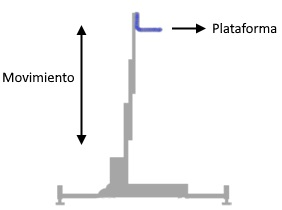
\includegraphics[width=2in]{imagenes/plataforma.jpg}
%\caption{Módulo elevador}
%\label{fig_plataforma}
%\end{figure}

\subsection{Pistón hidráulico}
Para simular el comportamiento de este actuador se consideró el modelo propuesto en \cite{Electro-hydraulic_actuator}. La planta es definida por un sistema no lineal, esta incluye un modelo de fricción, de una servo válvula y la dinámica de un cilindro externo que representa la carga. El esquema de la Figura \ref{fig_esquemapiston} describe físicamente el actuador considerado. Cada pistón cuenta con una cámara dividida por un émbolo, se bombea fluido desde $u_2$, por simplicidad consideraremos este flujo constante. La electro válvula $u$ controla el flujo para cada una de las cámaras $A$ y $B$, la diferencia de presión entre estas y el peso de la carga definirá el movimiento y la posición del pistón. 

\begin{figure}[!t]
	\centering
	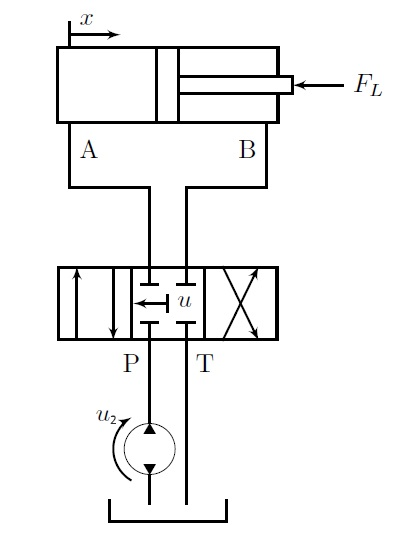
\includegraphics[width=2.3in]{imagenes/esquemapiston.jpg}
	\caption{Esquema físico}
	\label{fig_esquemapiston}
\end{figure}

En este trabajo se diseñó un control robusto para llevar el error de posición a cero asumiendo que el vector de estados es completamente medible. Las ecuaciones de estado que resultan son las mostradas en \ref{eq_statespace}, dónde $x_1$ y $x_2$ son la posición y velocidad del pistón respectivamente, $x_3$ es la presión de la carga, $x_4$ y $x_5$ son la dinámica y el control de la servo válvula.

\begin{eqnarray}
\label{eq_statespace}
\dot{x}_1&=&x_2\\
\nonumber \dot{x}_2&=&\frac{1}{m}(-k_sx_1-b_dx_2+\Lambda_ax_3-Fr-M)\\ 
\nonumber \dot{x}_3&=&-\alpha x_2-\beta x_3+(\gamma \sqrt{Ps-sgn(x_4)x_3})x_4\\
\nonumber \dot{x}_4&=&x_5\\
\nonumber \dot{x}_5&=&-c_nx_4-b_nx_5+a_nu
\end{eqnarray}

Los valores de los parámeros del modelo usados para simulación son presentados en la Tabla \ref{tab_valoresmodelo}. Con estos valores la respuesta del pistón es estable. Adicionalmente el sistema se configuró en lazo cerrado  y se agregó un control proporcional e integral, con el fin de que el sistema tenga error cero al estabilizarse y coincida con el valor de referencia que será el correspondiente al consensus.












\section{Consensus}


En muchos problemas que involucran múltiples agentes que requieren interactuar en una secuencia de tareas, típicamente las tareas y las interacciones pueden ser definidas por actividades en secuencias de tiempo que cada agente debe cumplir en determinado tiempo con recursos definidos, aunque estos problemas pueden ser solucionados con algoritmos de planeación, pueden ocurrir cambios durante la ejecución que harán que la tarea no se complete exitosamente, por tanto es e interés un marco de trabajo que cuando ocurran perturbaciones pueda adaptativamente sugerir cambios en los agentes  que permitan que lleguen a un acuerdo.   \cite{Decentralized_adaptive_scheduling}.

Cuando múltiples vehículos concuerdan en el valor de una variable de interés, se dice que han llegado a un \textit{consensus}, para lograr llegar a este estado, los vehículos deben compartir información en una red, además de tener algoritmos llamados algoritmos de consensus, los cuales negociarán como se llega a la variable deseada  \cite{DistributedConsensusinMulti}

La interacción de agentes en una red con cierta topología es representada por un grafo $G=(V,E)$ con el grupo de nodos $V=\{ 1,2,\ldots,n\}$ y bordes $E\subseteq V \times V$. Los vecinos del agente $i$ son definidos por $N_i=\{j \in V :(i,j)\in E\}$.


\subsection{Information Consensus}
Consideremos una red de agentes con dinámicas $\dot{x}_i=u_i$ interesados en alcanzar un consensu mediante comunicación local con sus vecinos en un grafo $G=(V,E)$. Alcanzar consensus significa que el sistema converge asintóticamente a $x_1=x_2=\ldots =x_n$, es decir que el los valores de cada agente serán $x=\alpha\textbf{1}$ dónde $\alpha \in \mathbb{R}$ es la desición colectiva del grupo de agentes. Sea $A=[a_{ij}]$ a matriz de adyacencia del grafo $G$. El conjunto de vecinos del agente $i$ es $N_i$ y está definido por $N_i=\{j\in V:a_{ij}\neq 0 \} \ \ \ V=\{1,2,\ldots,n \}$.

Note que $a_{ij}>0$ (es vecino) cuando $(i,j)\in E$, de otro modo $a_{ij}=0$. El agente $i$ se comunica con el agente $j$ si $j$ es un vecino.
Estableciendo $a_{ij}=0$ define el hecho que el vehículo $i$ no puede recibir información desde el vehículo $j$. 
El conjunto de todos los nodos y sus vecinos define el borde $E$ del grafo. 

\begin{equation}
\dot{x}_i(t)=\sum_{j\in N_i}a_{ij}(x_j(t)-x_i(t))
\label{eq_consensusinformation}
\end{equation}

El sistema lineal definido en \ref{eq_consensusinformation} es un algoritmo distribuido de consensus, este garantiza convergencia a una decisión colectiva mediante interacción local entre agentes \cite{DistributedConsensusinMulti} \cite{Olfati-saber07consensusand} \cite{Ordonez2014} \cite{Decentralized_adaptive_scheduling}.
Una consecuencia de \ref{eq_consensusinformation} es que la información del estado $x_i(t)$ del vehículo $i$ es llevado hacia la información del estado de sus vecinos.
Asumiendo que el grafo es unidireccional, es decir $a_{ij}=a_(ji)$ para todo $i,j$, esto conlleva a que la suma de los estados de todos los nodos es una cantidad invariante, o $\sum_i\dot{x}_i=0$, aplicando esta condición dos veces en $t=0$ y en $t=\infty$ se obtiene que:
\begin{equation}
\alpha=\frac{1}{n}\sum_{i}x_i(0)
\end{equation}

Esto puede ser interpretado como que el valor de consensus al que llegarán los agentes será el promedio de los valores iniciales de cada uno.


\subsection{Consensus Tracking Protocol}
En algunas aplicaciones es deseable que el estado de consensus de información converja a un valor predefinido. Por tanto los agentes deben converger a un mismo valor, pero también al estado de su valor de referencia. Por tanto se considera un grupo de $n$ agentes más un líder virtual $n+1$. El estado $x_{n+1}$=$x_r \in \mathbb{R}^n$ contiene la información de referencia para el consensus.
El grafo $G_{n+1}=(V_{n+1},E_{n+1})$ es usado para modelar la interacción entre $n+1$ vehículos (con el líder virtual). Definamos $A_{n+1}=[a_{ij}] \in \mathbb{R}^{n+1\times n+1}$ la matriz de adyacencia asociada a $G_{n+1}$, dónde $a_{ij}>0$ si $(j,i)\in E_{n+1}$ y $a_{n+1}>0$ si $x_r$ está disponible para el vehículo $i$ para $i=1,2,\ldots,n$. Finalmente, $a_{(n+1)j}=0$ para todo $j=1,2,\ldots,n+1$ y $a_ii=0$ para todo $i=1,2,\ldots,n.$. El líder puede ser interpretado como un nodo que ignora todos los demás nodos, pero continua transmitiendo su información.

De \cite{Ordonez2014}(Theorem1) supone que $A_{n+1}$ es constante. El problema de \textit{Consensus Tracking} conuna referencia constante es resuelto con la definición del líder virtual, si y sólo si el grafo $G_{n+1}$ tiene un árbol de alcance directo (\textit{directed spanning tree})

Note que el vehículo $n+1$ posee la información de la referencia y la condición que $G_{n+1}$ tiene un árbol de alcance directo es equivalente a la condición que al menos, un camino une a todos los vehículos, incluyendo al líder virtual $n+1$.






\section{Restricciones}


Las restricciones para el sistema representan una condición importante debido a que si no se cumplen podría fallar todo el funcionamiento. Una manera de abordar este requerimiento es desde el punto de vista de optimización, visualizando el consensus cómo la minimización de a distancia entre agentes  y en la cual se llega a la solución mediante el método del gradiente descendente ya que se tiene unas dinámicas de la forma $\dot{x}=-\nabla_xf(x)$. Vamos entonces a considerar los métodos de barrera para una optimización con restricciones, la región factible está definida por\\
$S=\{x\in \mathbb{R}^n : g_i(x)\leq 0, i=1,\ldots,n \}$\\
En los métodos de barrera se asume que es dado un punto $x^0$ que está dentro de la región factible $S$, y nosotros imponemos un alto costo en los puntos dentro de la región factible que están cerca al borde, creando así una barrera para dejar la región factible \cite{barriermethods_epelman}.

Una función barrera es cualquier función continua $b(x)$ definida en el interior de la región factible $S$ tal que $b(x)\rightarrow +\infty$ cuando $g_i(x) \rightarrow 0^-$.\cite{Nonlinear_Programming_zorning}  Dos ejemplos comunes para funciones de barrera son\\
\begin{equation}
b(x)=-\sum_{i=1}^{n}ln(-g_i(x)) \ \ \ \textnormal{y} \ \ \ b(x)=-\sum_{i=1}^{n}\frac{1}{g_i(x)}
\label{eq_barriermethods}
\end{equation}

Note que ahora el problema no tiene restricciones, y la desigualdad $g(x)<0$ está definida en el dominio de la función objetivo.

Para nuestro caso en particular la restricción radica en que las plataformas de elevación podrán desalinearse máximo $1mm$, por tanto la función de barrera diseñada es
\begin{equation}
b(x)=\sum_{i=1}^{n}\sum_{j=1}^{n}\frac{b_a}{1-(x_i-x_j)}; \forall j\neq i
\end{equation}





\section{Ensamble modelo real}


El consensus contiene las dinámicas de los agentes y es posible conocer la evolución de las trayectorias, pero estos valore son ideales. La implementación de dicho algoritmo en un sistema real deberá tener en cuenta las dinámicas propias de cada agente. En este escenario los valores resultado del consensus serán los valores de referencia para los agentes(actuadores) como se observa en la Figura \ref{fig_consensus_piston}. El sistema real debe ser estable y llegar a un valor de referencia dado. Por ejemplo para nuestro caso el actuador es un pistón hidráulico con un controlador proporcional integral que sigue un valor de referencia.

\begin{figure}[!h]
\centering
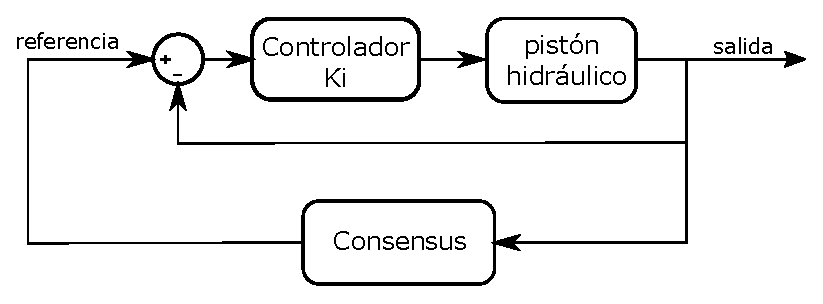
\includegraphics[width=3in]{imagenes/consensus_piston.eps}
\caption{Esquema de conexión Consensus-Planta}
\label{fig_consensus_piston}
\end{figure}

Las dinámicas de cambio del consensus idealmente deben ser más lentas que las del sistema físico con el objetivo de que la planta pueda seguir la trayectoria trazada por el consensus. Para efectos prácticos de la implementación desde el punto de vista discreto el periodo del consensus deberá ser mayor que el de la planta. Para que exista una mejor interacción consensus-planta, el valor de entrada para cada iteración del consensus será el valor de posición de la planta (ver Figura \ref{fig_consensus_piston}), esto conlleva a que si los actuadores son lentos, el consensus "espere" a la planta, pero si la planta es sufucientemente rápida la planta no influirá en el comportamiento del consensus.




\section{Simulaciones}


Para realizar las simulaiones se tomaron los datos correspondientes al modelo del pistón de \cite{Electro-hydraulic_actuator}, los cuales se muestran en la Tabla \ref{tab_valoresmodelo}. 


\begin{center}
	\captionof{table}{Valores del Modelo}
	\label{tab_valoresmodelo} 
	\begin{tabular}[t]{clccl}
		$m$ & $24kg$ & & $k_s$ & $1610 N/m$\\
		$b_d$ & $310N/(m/s)$ & & $Ps$ & $1.03e7 pa$\\
		$\Lambda_a$ & $3.26e-4 m^2$ & & $\alpha$ & $1.51e10 N/m^3$\\
		$\beta$ & $1 1/s$ & & $\gamma$ & $7.28e8 g^{0.5}/m^{1.5}s^2$\\
		$M$ & $300-500 N$ & & $a_n$ & $2.4315e5$\\
		$b_n$ & $6.2529e2$ & & $c_n$ & $2.5676e5$
	\end{tabular}
\end{center}

La posición inicial para cada agente es $[0,0.1,0.2,0.3,0.4,0.5]$, el periodo de consensus $T_c=0.5 [s]$, matriz de adyacencia es uan martriz de unos con ceros en la diagonal (fully connected),los valores iniciales de las demás variables de estado para todos los actuadores es $[0,6e6,0,0]$, los valores de carga para cada actuador $[300,300,310,350,590,700]$, los valores de las constantes del controlador son $k_p=1e-2$ y $k_i=1e-6$, el periodo de solución para la planta $T_s=0.1 [s]$, el valor del numerado de la función barrera $b_a=1e-3$ valore de referencia para el consensus $0.7$  y finalmente el tiempo total de la solución es $40 [s]$.


\begin{figure}[!h]
	\centering
	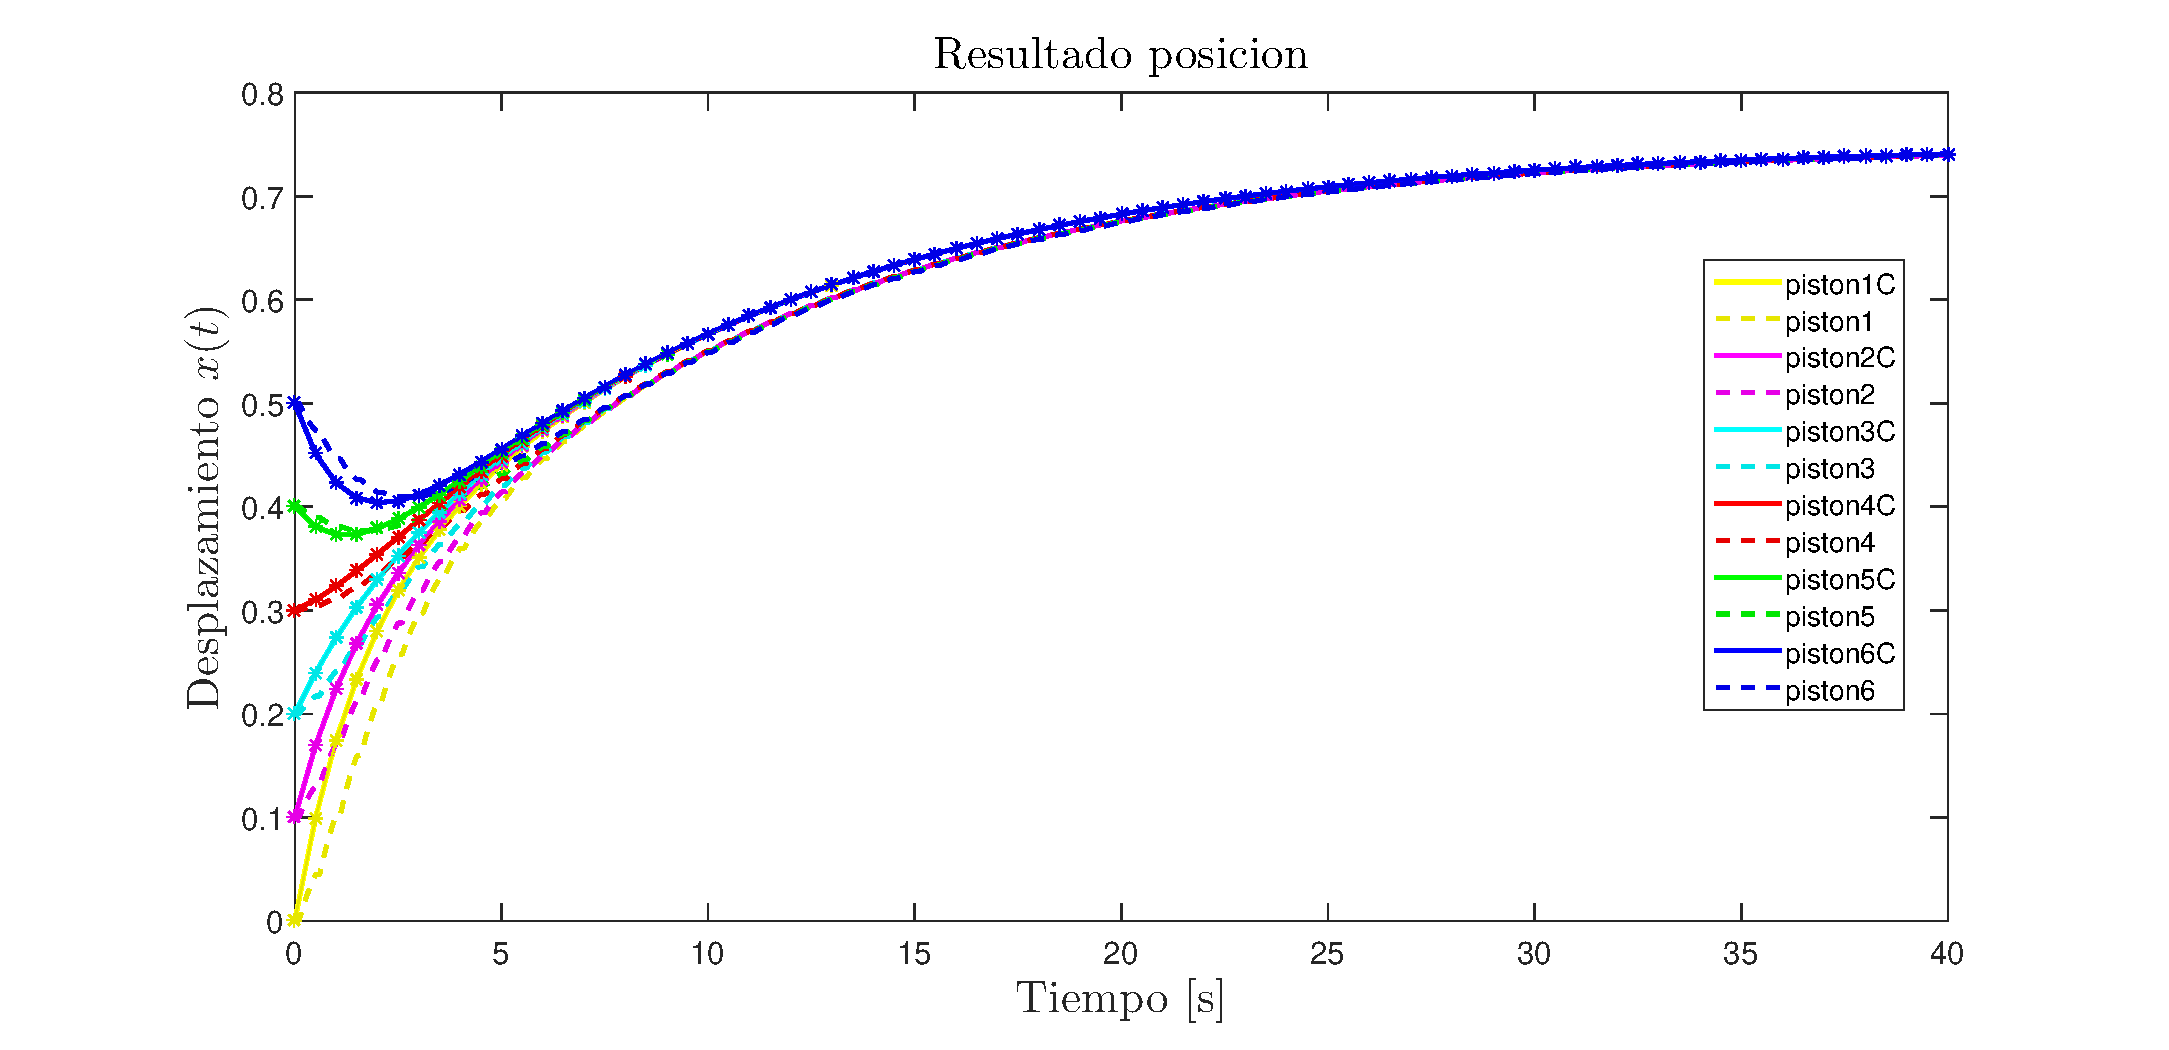
\includegraphics[width=3.9in]{imagenes/consensus_pos.eps}
	\caption{Consensus en tiempo}
	\label{fig_consensus_pos}
\end{figure}
El resultado es como el esperado, se pueden diferenciar dos dinámicas en el resultado de la Figura \ref{fig_consensus_pos}, donde  primero se trata de minimizar las diferencias entre agentes y a medida que se van acercando comienzan a converger en grupo al valor de referencia del consensus, observamos que las posiciones reales (líneas punteadas) siguen con los valores de referencia de manera suave por tanto los periodos para cada sistema son los adecuados.

\begin{figure}[!h]
	\centering
	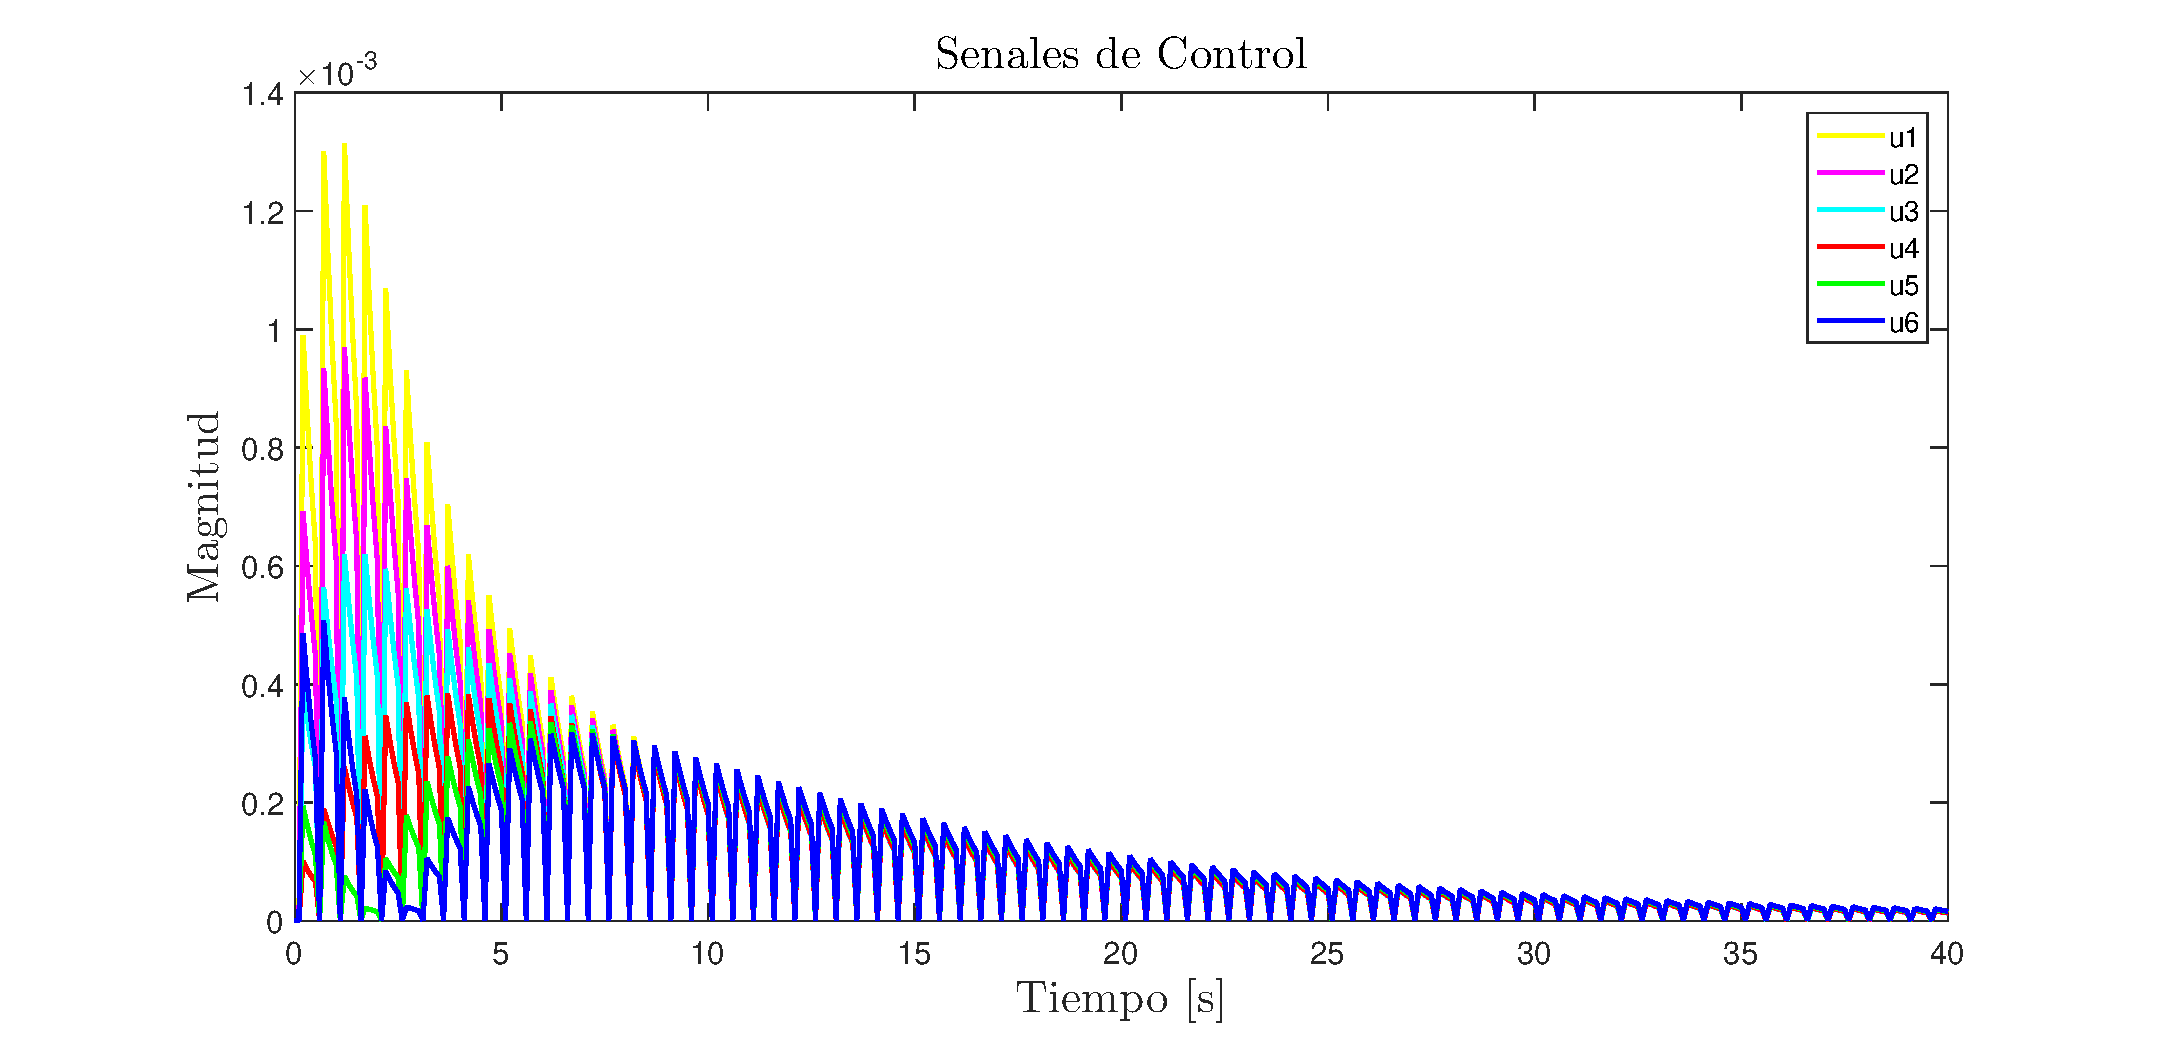
\includegraphics[width=3.9in]{imagenes/senales_conrtrol.eps}
	\caption{Señales de Control en tiempo}
	\label{fig_senales_conrtrol}
\end{figure}

Las señales de control Figura \ref{fig_senales_conrtrol} más altas inicialmente son las de los agentes más lejanos al punto de encuentro. Una vez los agentes confluyen a la misma posición, en su recorrido grupal al valor de referencia, las señales de control son las mismas y van disminuyendo a medida que convergen, el cual es el comportamiento esperado.

\begin{figure}[!h]
	\centering
	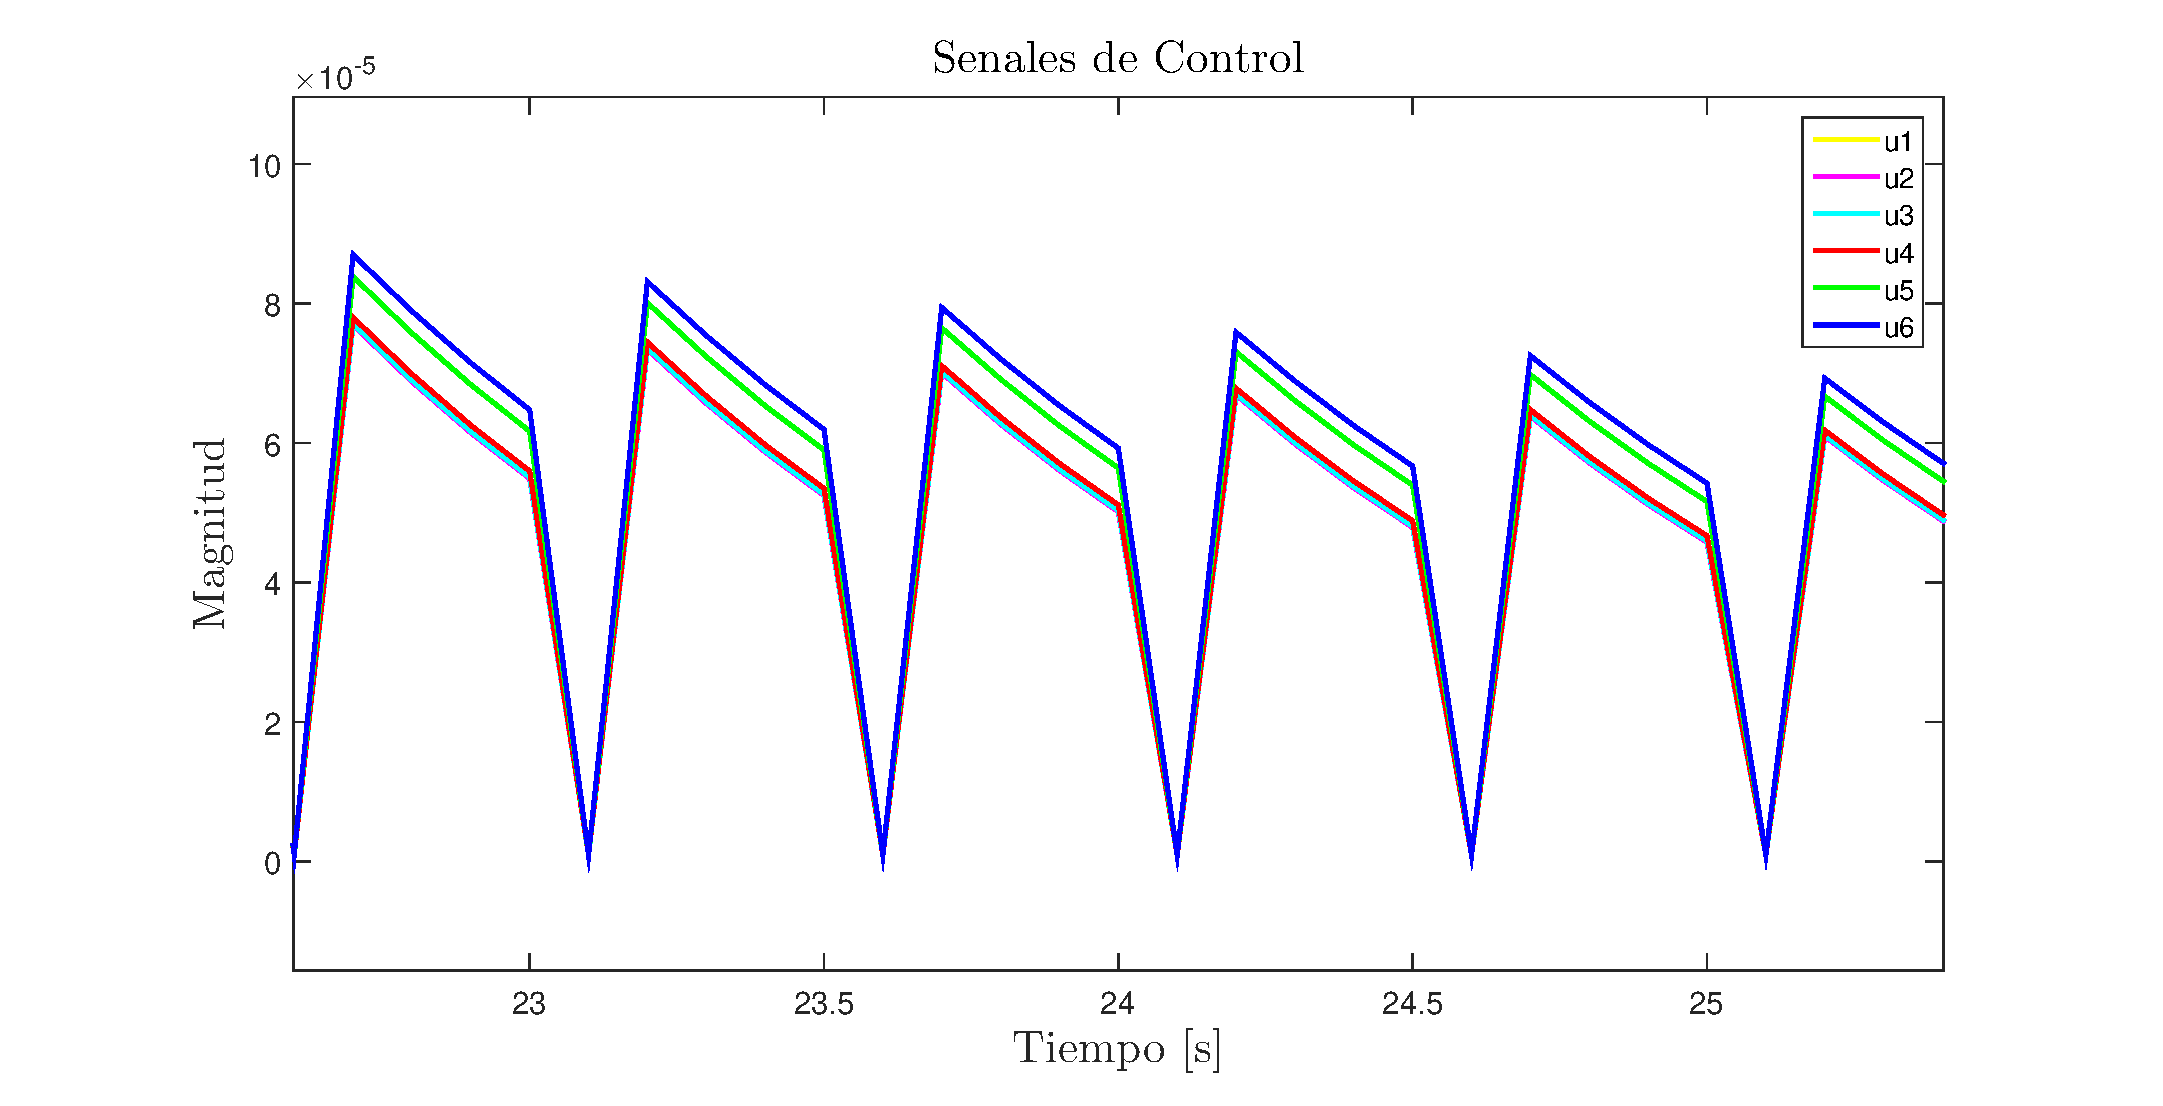
\includegraphics[width=3.9in]{imagenes/senales_conrtrol_zoom.eps}
	\caption{Zoom Señales de Control en tiempo}
	\label{fig_senales_conrtrol_zoom}
\end{figure}
En la Figura \ref{fig_senales_conrtrol_zoom} se evidencian algunas diferencias en las señales de control, esto corresponde a las diferentes caras que tiene cada actuador, vemos que las señales más altas corresponden a los actuadores que tienen más peso sobre ellos, por tanto las dinámicas propias del consensus hacen que se equilibren estas diferencias.

\begin{figure}[!h]
	\centering
	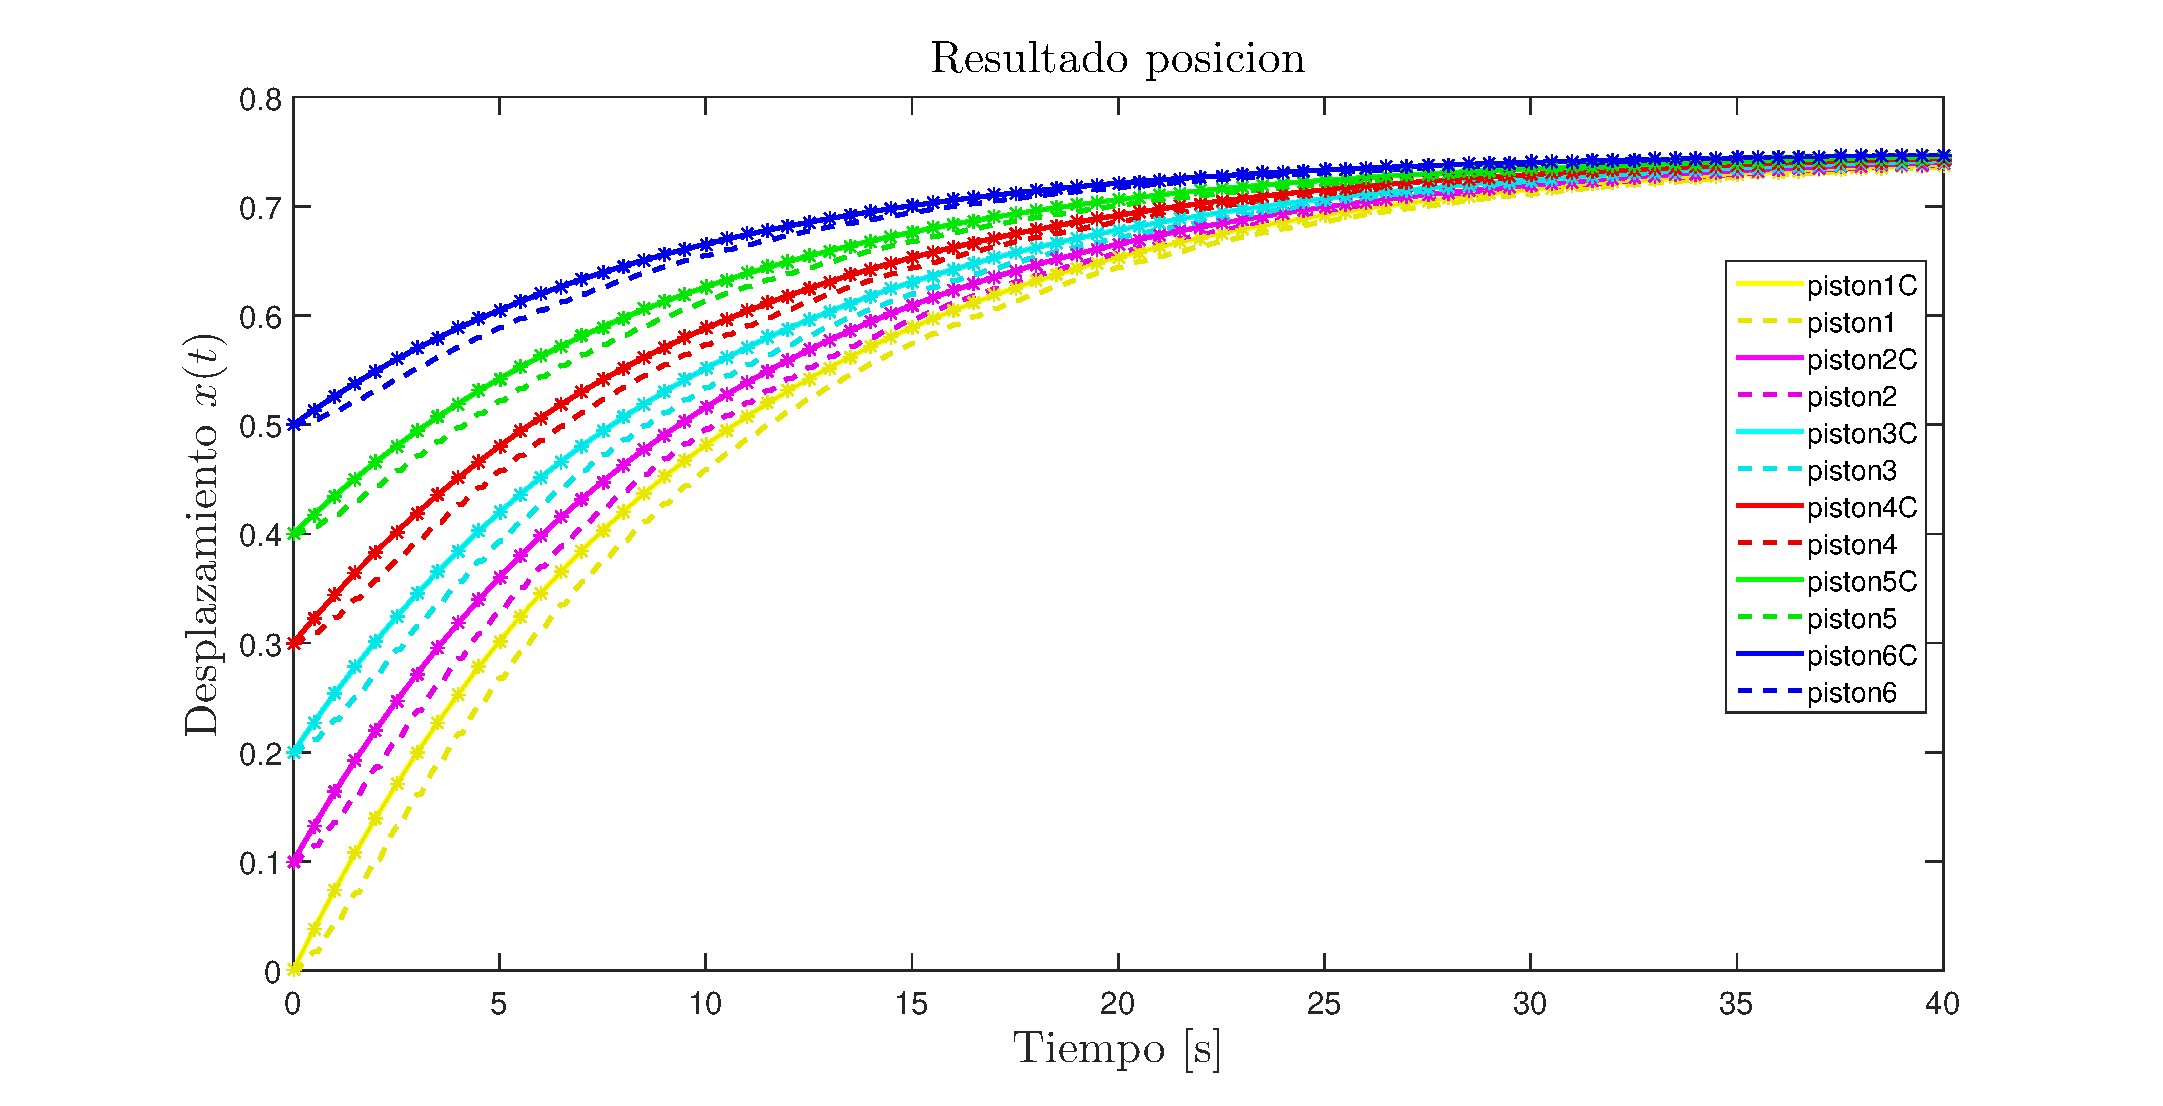
\includegraphics[width=3.9in]{imagenes/consensus_pos_min.eps}
	\caption{Consensus en tiempo para un grafo mínimamente conectado}
	\label{fig_consensus_pos_min}
\end{figure}
En la Figura \ref{fig_consensus_pos_min} se muestra el resultado para el sistema cuando el grafo justo cumple la condición de ser un árbol de alcance directo, es decir los agentes no se conectan entre ellos, sólo se conectan con el líder virtual. El resultado confirma que que se llega a un consensus en el valor de referencia, pero sus dinámicas cambian, solo dependen de la referencia.

\begin{figure}[!h]
	\centering
	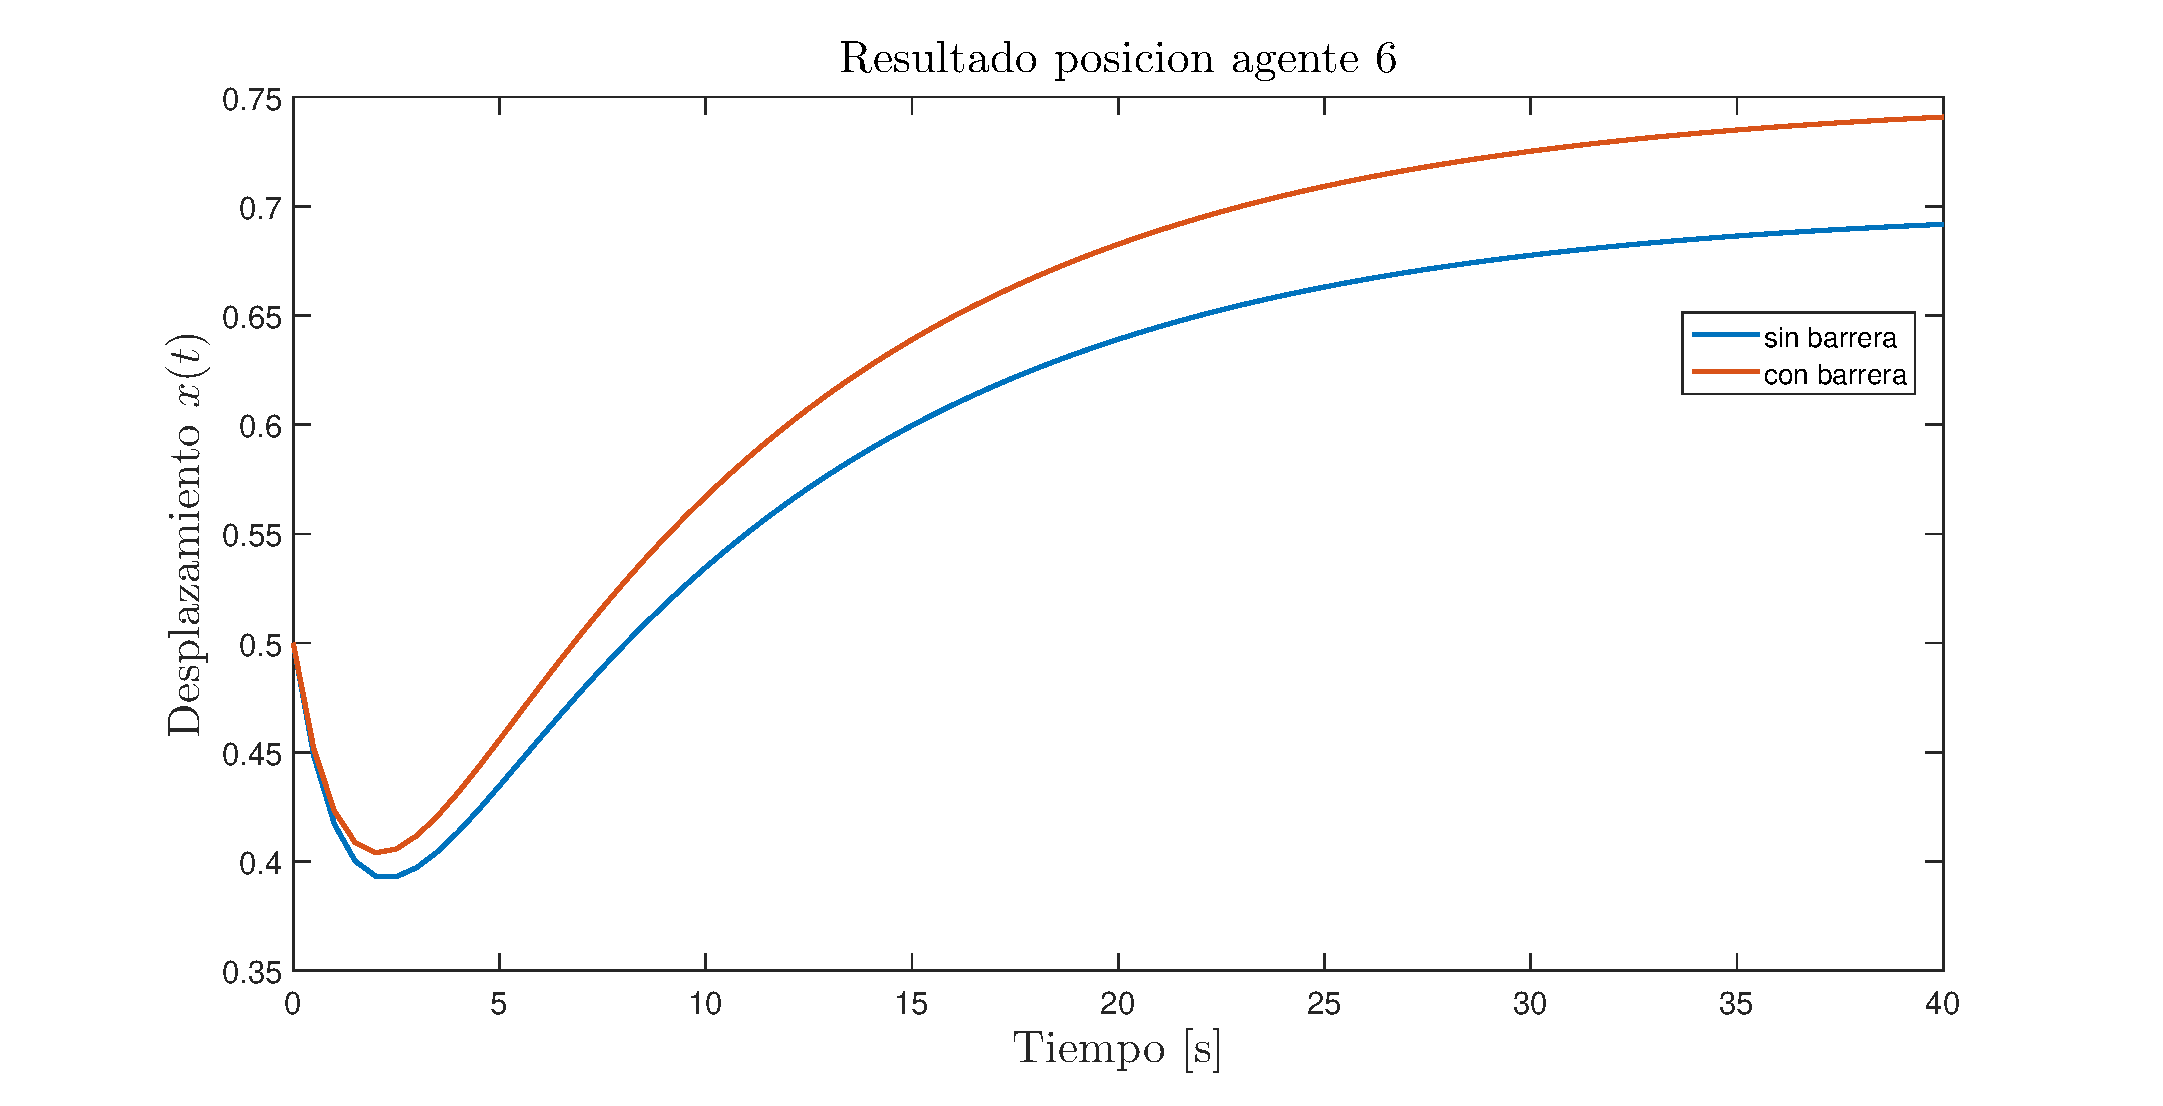
\includegraphics[width=3.9in]{imagenes/efecto_barrera.eps}
	\caption{Trayectoria del agente 6 con y sin barrera}
	\label{fig_efecto_barrera}
\end{figure}
En la Figura \ref{fig_efecto_barrera} se muestra e comportamiento de uno de los agentes con y sin la presencia de la restricción. Se evidencia que cunado la restricción está activa las dinámicas son más rápidas, y este efecto aumentará a medida que el sistema se acerque a los valores de la restricción.



% An example of a floating figure using the graphicx package.
% Note that \label must occur AFTER (or within) \caption.
% For figures, \caption should occur after the \includegraphics.
% Note that IEEEtran v1.7 and later has special internal code that
% is designed to preserve the operation of \label within \caption
% even when the captionsoff option is in effect. However, because
% of issues like this, it may be the safest practice to put all your
% \label just after \caption rather than within \caption{}.
%
% Reminder: the "draftcls" or "draftclsnofoot", not "draft", class
% option should be used if it is desired that the figures are to be
% displayed while in draft mode.
%
%\begin{figure}[!t]
%\centering
%\includegraphics[width=2.5in]{myfigure}
% where an .eps filename suffix will be assumed under latex, 
% and a .pdf suffix will be assumed for pdflatex; or what has been declared
% via \DeclareGraphicsExtensions.
%\caption{Simulation results for the network.}
%\label{fig_sim}
%\end{figure}

% Note that the IEEE typically puts floats only at the top, even when this
% results in a large percentage of a column being occupied by floats.


% An example of a double column floating figure using two subfigures.
% (The subfig.sty package must be loaded for this to work.)
% The subfigure \label commands are set within each subfloat command,
% and the \label for the overall figure must come after \caption.
% \hfil is used as a separator to get equal spacing.
% Watch out that the combined width of all the subfigures on a 
% line do not exceed the text width or a line break will occur.
%
%\begin{figure*}[!t]
%\centering
%\subfloat[Case I]{\includegraphics[width=2.5in]{box}%
%\label{fig_first_case}}
%\hfil
%\subfloat[Case II]{\includegraphics[width=2.5in]{box}%
%\label{fig_second_case}}
%\caption{Simulation results for the network.}
%\label{fig_sim}
%\end{figure*}
%
% Note that often IEEE papers with subfigures do not employ subfigure
% captions (using the optional argument to \subfloat[]), but instead will
% reference/describe all of them (a), (b), etc., within the main caption.
% Be aware that for subfig.sty to generate the (a), (b), etc., subfigure
% labels, the optional argument to \subfloat must be present. If a
% subcaption is not desired, just leave its contents blank,
% e.g., \subfloat[].


% An example of a floating table. Note that, for IEEE style tables, the
% \caption command should come BEFORE the table and, given that table
% captions serve much like titles, are usually capitalized except for words
% such as a, an, and, as, at, but, by, for, in, nor, of, on, or, the, to
% and up, which are usually not capitalized unless they are the first or
% last word of the caption. Table text will default to \footnotesize as
% the IEEE normally uses this smaller font for tables.
% The \label must come after \caption as always.
%
%\begin{table}[!t]
%% increase table row spacing, adjust to taste
%\renewcommand{\arraystretch}{1.3}
% if using array.sty, it might be a good idea to tweak the value of
% \extrarowheight as needed to properly center the text within the cells
%\caption{An Example of a Table}
%\label{table_example}
%\centering
%% Some packages, such as MDW tools, offer better commands for making tables
%% than the plain LaTeX2e tabular which is used here.
%\begin{tabular}{|c||c|}
%\hline
%One & Two\\
%\hline
%Three & Four\\
%\hline
%\end{tabular}
%\end{table}


% Note that the IEEE does not put floats in the very first column
% - or typically anywhere on the first page for that matter. Also,
% in-text middle ("here") positioning is typically not used, but it
% is allowed and encouraged for Computer Society conferences (but
% not Computer Society journals). Most IEEE journals/conferences use
% top floats exclusively. 
% Note that, LaTeX2e, unlike IEEE journals/conferences, places
% footnotes above bottom floats. This can be corrected via the
% \fnbelowfloat command of the stfloats package.




\section{Conclusion}
aqui concluimos



% conference papers do not normally have an appendix

% trigger a \newpage just before the given reference
% number - used to balance the columns on the last page
% adjust value as needed - may need to be readjusted if
% the document is modified later
%\IEEEtriggeratref{8}
% The "triggered" command can be changed if desired:
%\IEEEtriggercmd{\enlargethispage{-5in}}

% references section

% can use a bibliography generated by BibTeX as a .bbl file
% BibTeX documentation can be easily obtained at:
% http://mirror.ctan.org/biblio/bibtex/contrib/doc/
% The IEEEtran BibTeX style support page is at:
% http://www.michaelshell.org/tex/ieeetran/bibtex/
%\bibliographystyle{IEEEtran}
% argument is your BibTeX string definitions and bibliography database(s)
%\bibliography{IEEEabrv,../bib/paper}
%
% <OR> manually copy in the resultant .bbl file
% set second argument of \begin to the number of references
% (used to reserve space for the reference number labels box)
%\begin{thebibliography}{1}
%
%\bibitem{IEEEhowto:kopka}
%H.~Kopka and P.~W. Daly, \emph{A Guide to \LaTeX}, 3rd~ed.\hskip 1em plus
%  0.5em minus 0.4em\relax Harlow, England: Addison-Wesley, 1999.
%
%\end{thebibliography}

\bibliographystyle{IEEEtran}
% argument is your BibTeX string definitions and bibliography database(s)
\bibliography{biblio}


% that's all folks
\end{document}


